This report presents a length-based assessment of the multi-species deep slope hook and line fisheries targeting snappers, groupers and emperors, at depths ranging from 50 to 500 meters, in fisheries management areas (WPP) 712 and 713 in the Java Sea and the Makassar Strait in Central Indonesia. These 2 WPP are here, as they are both part of a continuous habitat and fishing ground where fleets freely operate in both WPP.

Drop line and long line vessels fish in this area together with a number of other gear types including bottom trawls that go under various names. Bottom long line vessels fish on the shelf area as well as on the top of the slopes that drop to deeper waters, mostly on and around the border between WPP 712 and WPP 713, where the Java Sea meets the Makassar Strait. Drop liners fish the deep slopes also to greater depths, mostly in the Makassar Strait. The drop line fishery is an active vertical hook and line fishery operating at depths from 50 to 500 meters, whereas long lines are set horizontally along the bottom at depths ranging from 50 to 150 meters. Trawlers and other net fisheries work mostly over the shallower parts of the Java Sea shelf area at depths that may possibly overlap with the long line fisheries only.

Various fleets are operating in this region, including medium sized long liners from Probolinggo in East Java and mostly small scale drop liners from all around the Makassar Strait. Vessels from several of these fleets contributed data to the current assessment. Some fleets based within this area, especially larger sized long liners from Probolinggo, operate in Eastern Indonesia in WPP 718 and 573. The data on catches from those fleets are not included in this report but instead used in the assessments of the fisheries in each respective WPP.

This report analyzes length frequencies of the 50 species of fish that were the most abundant in the combined drop and long line fisheries operating in WPP 712 and WPP 713. For a complete overview of the species composition please refer to the ID guide prepared for these fisheries:

\textbf{CLICK: }\href{http://goo.gl/kTSGTJ}{Link to on-line E-Book Species ID Guide}

For further background on species life history characteristics, and data-poor length based assessment methods, as applied in this report, please refer to the assessment guide that was separately prepared for these fisheries:

\textbf{CLICK: }\href{http://goo.gl/HLNC4q}{Link to on-line E-Book Assessment Guide with Biological Information}

Data in this report represent complete catches by small and medium scale vessels from the above described fleets. All fish captured were photographed on measuring boards by fishing crew participating in our Crew Operated Data Recording System or CODRS. Images were analyzed by project staff to generate the species specific length frequency distributions of the catches which served as the input for our length based assessment.

\begin{center}
\graphicspath{{/root/R-project/IFishSnapperWPP712_713/Images/}}
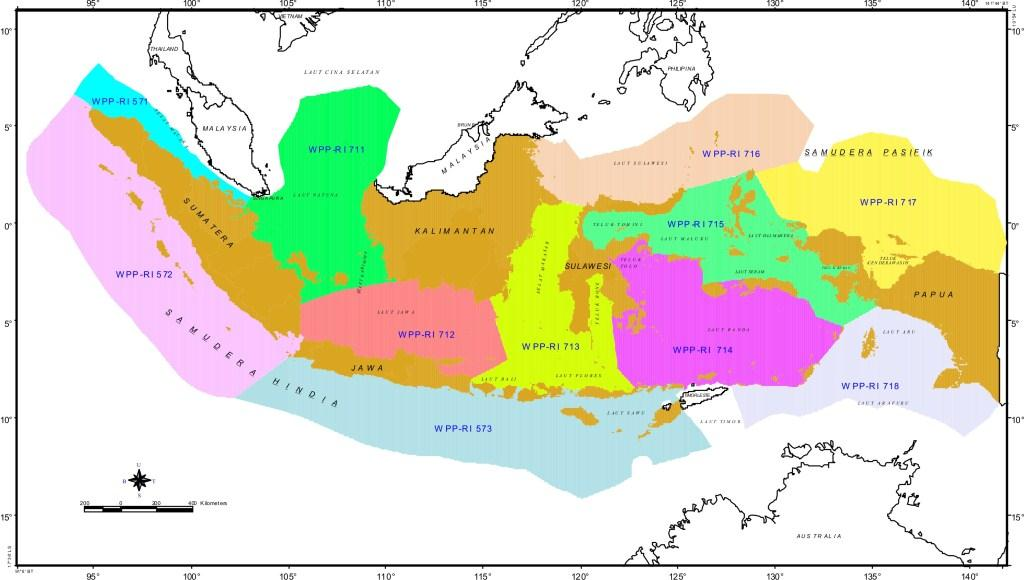
\includegraphics[scale=1.8]{wpp-indonesia.jpg}

Figure 1. Fisheries Management Areas (WPP) in Indonesian marine waters.
\end{center}

\begin{center}
\graphicspath{{/root/R-project/IFishSnapperWPP712_713/Images/}}
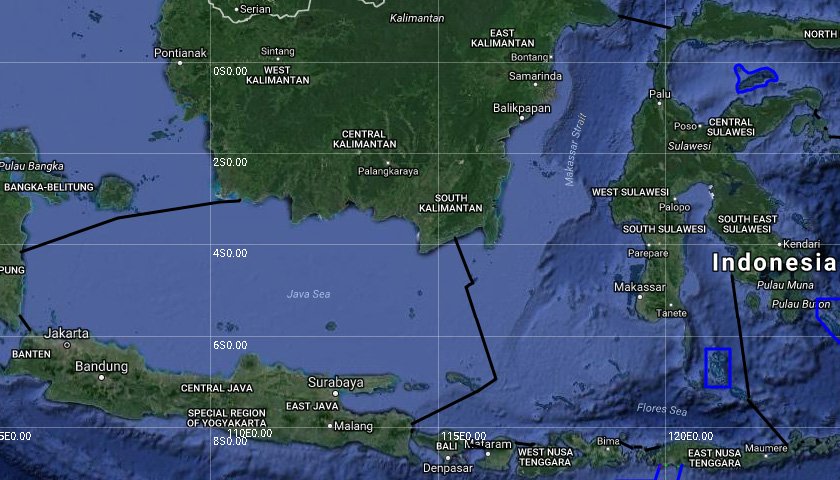
\includegraphics[scale=0.5]{AreaB-Satellite.jpg}

Figure 2. Bathymetric map of the Java Sea and the Makassar Strait, WPP 712 and WPP 713, in Central Indonesia. Black lines are WPP boundaries, blue lines are MPAs.
\end{center}